% ====================================================
%   Copyright (C)2019 All rights reserved.
%
%   Author        : Xin-Xin Ma
%   Email         : xxmawhu@163.com
%   File Name     : appendix_ds.tex
%   Last Modified : 2019-10-27 15:02
%   Describe      :
%
% ====================================================%
\chapter{关于$D_{s}^{+} \to p \bar{p} e^{+} \nu_{e}$的分析}
\section{分支比和形状因子}
在这个小节,我们将讨论形状因子大小和分支比之间的关系。假设$p\bar{p}$对来自
于中间共振态$X$,$X$是一个赝标量粒子。采取单极点模型,衰变的分宽度振幅的形式是
\begin{equation}
    \frac{d \Gamma (D_{s}^{+} \rightarrow X e^{+} \nu _{e} )}{d q^{2}}
    = \frac{G^{2}_{F} \cdot | V_{cs} |^{2} p_{X} ^{3} }{24 \pi ^{3}} f
    _{X} (q^{2}){}^{2}
\end{equation}
其中$G_{F}$为费米常数,$|V_{cs}|$为CKM矩阵元,$p_{X}$为共振态在$D_{s}^{+}$质心系下的动量大小,$q$是转移动量为$D_{s}^{+}$
和$X$的动量的差,
$f_{+}(q^{2})$是形状因子。我们采用单极点模型来描述$f_{+}(q^{2})$~\cite{Bauer:1988fx},其形式为
\begin{equation}
    f_{+}(q^{2}) = \frac{f_{0}}{1-\frac{q^{2}}{M_{pole}^{2}}},
\end{equation}
其中$M_{pole} = m_{D_{s}^{*+}}$。
考虑到衰变道 $D_{s}^{+} \to \eta e^{+} \nu_{e}$ 和
$ D_{s}^{+} \to X(p\bar{p}) e^{+} \nu_e{e}$ 之间的高度相似性,
我们首先估算了两者分支比的比值,定义如下
\begin{equation}
   R =  \frac{Br(D_{s}^{+} \rightarrow X(p\bar{p}) e^{+} \nu_{e})}
    {Br(D_{s}^{+} \to \eta e^{+} \nu_{e}) } 
\end{equation}
利用$Br(D_{s}^{+} \to \eta e^{+} \nu_{e}) = (2.67 \pm 0.29) \%$~\cite{PDG},对于
每一对的输入值,我们就能预言$Br(D_{s}^{+} \to \eta e^{+} \nu_{e})$。
\begin{figure}[htbp]
    \centering
    \begin{subfigure}[]{0.45\textwidth}
        \begin{center}
            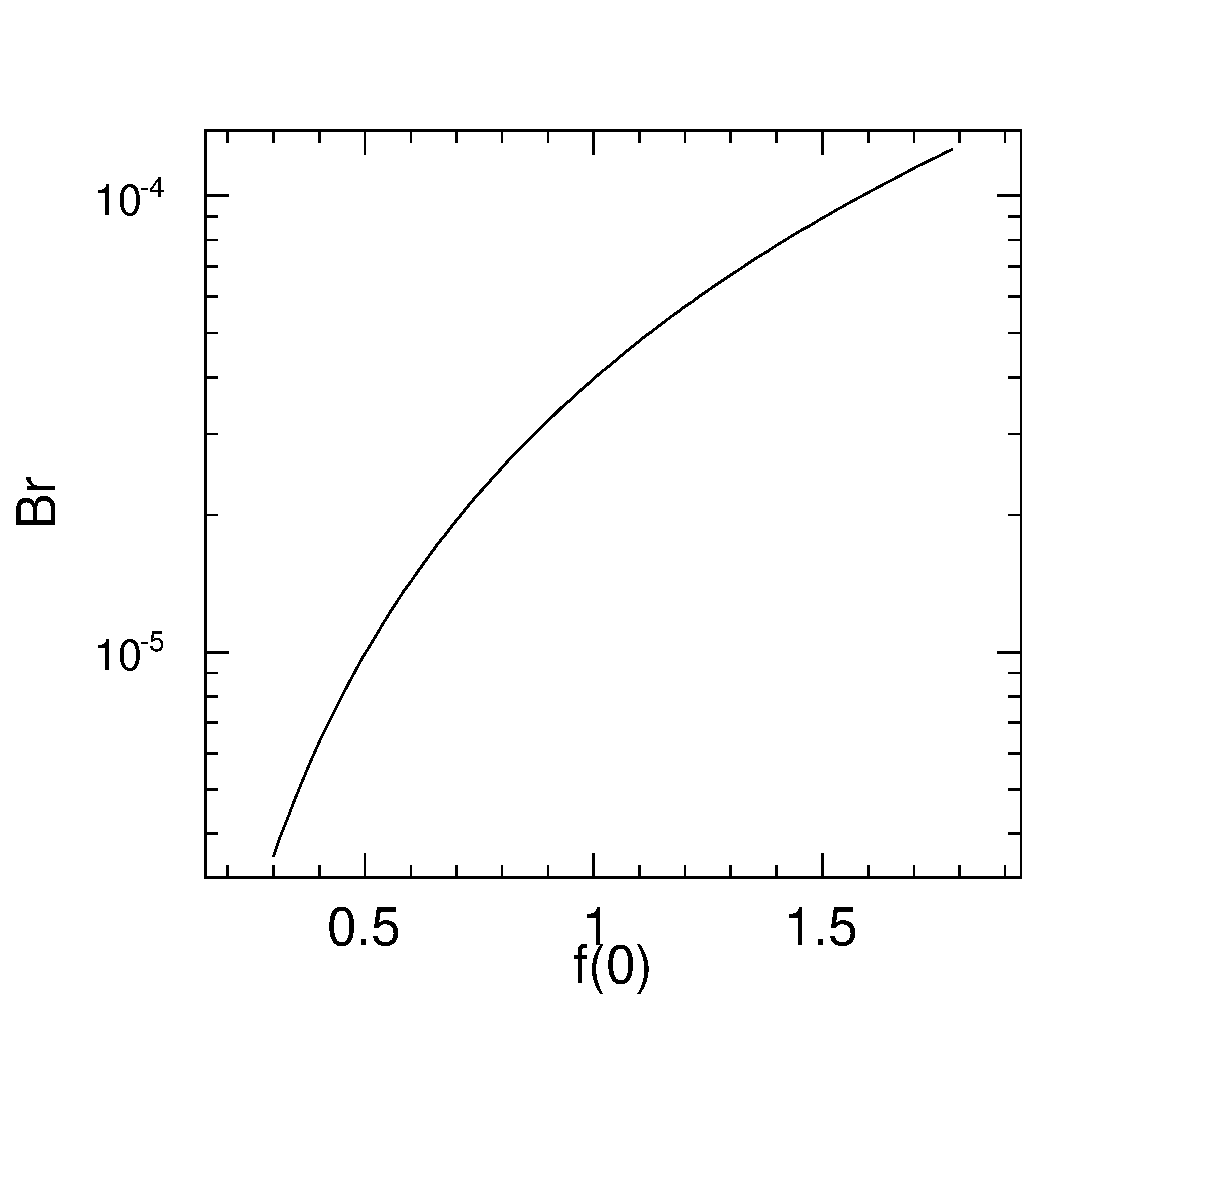
\includegraphics[width=1.0\linewidth]{dsToPPbar/f_0.eps}
        \end{center}
        \caption{}%
        \label{fig:}
    \end{subfigure}
    \begin{subfigure}[]{0.45\textwidth}
        \begin{center}
       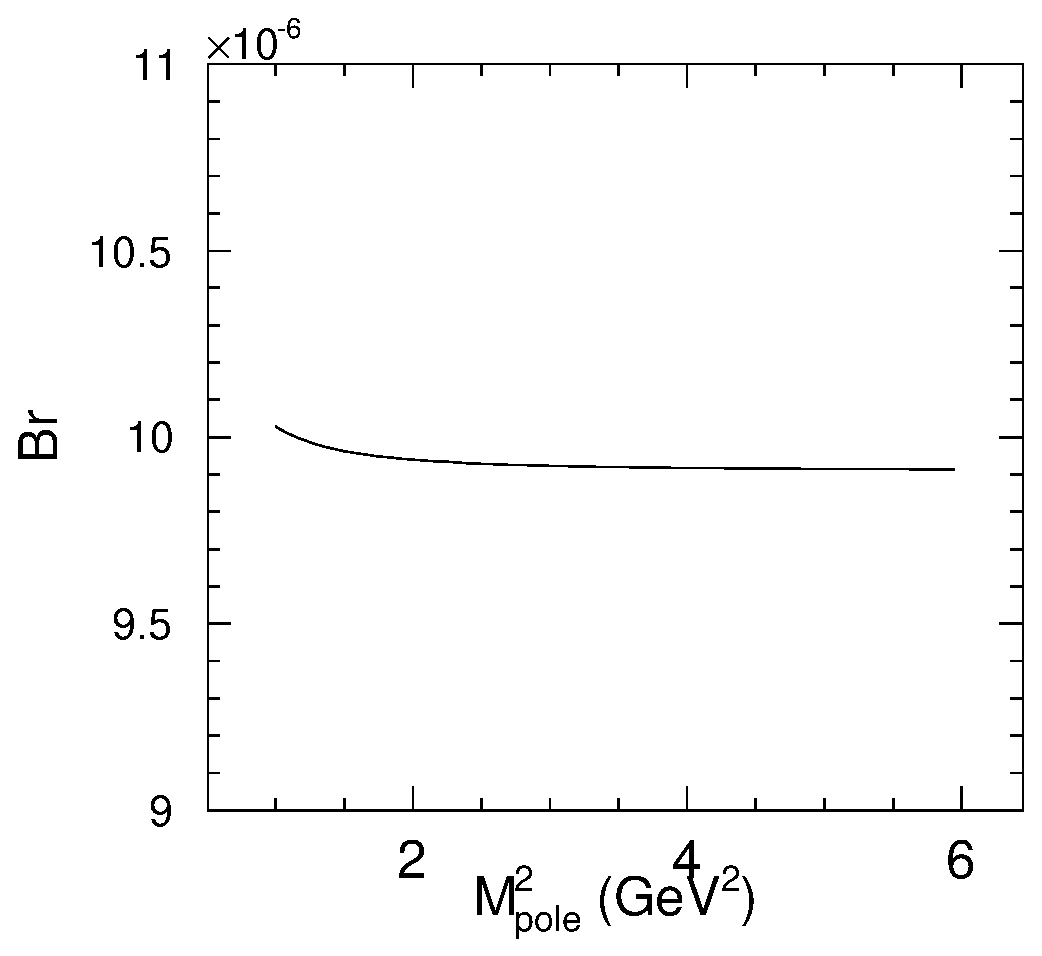
\includegraphics[width=1.0\linewidth]{dsToPPbar/m_pole}
        \end{center}
        \caption{}%
        \label{fig:}
    \end{subfigure}
    
    \caption{浮动参数 $f(0)$ 和 $M_{pole}^{2}$}%
    \label{fig:float_parameter}
\end{figure}
如图\ref{fig:float_parameter}所示,参数$M_{pole}$的取值对分支比的值影响极小,
另一个参数$f_{0}$起主导作用。如果我们假定$f_{0}=1$,相应的分支比大小为
\begin{equation}
Br(D_{s}^{+} \rightarrow X(p\bar{p}) e^{+} \nu_{e}) \sim 10^{-5}.
\end{equation}
    
\section{质子鉴别的系统误差研究}
为了研究质子重建的系统误差,我们必须要选择一个控制样本。由于2016年BESIII对
探测器的飞行时间计数器 (TOF)进行了重大升级,首次的取数恰好在4178MeV能量点,
我们只能选取连续区的
$e^{+} e^{-} \rightarrow p \bar{p} \pi^{+} \pi^{-}$ 
事例作为控制样本。
\subsection{效率的定义}
粒子鉴别的效率$\epsilon_{pid}$的定义为
\begin{equation}
    \epsilon_{pid} = \frac{n}{N}
\end{equation}
其中分母$N$是控制样本的质子(或反质子)的总数,分子$n$是这些候选质子(反质子中
通过粒子鉴别程序被成功鉴别为质子的个数. 考虑到效率大小约为99\%,常用的误差计算
公式已经失效,为此并利用文献\cite{brown2001interval}中的公式
来计算$\epsilon_{pid}$的误差。具体的程序借助于了\textbf{ROOT}提供的
类\textbf{TGraphAsymmErrors},这里不再详细叙述计算程序的细节。
按上文的叙述,我们将分别得到在数据和蒙特卡洛样本中质子鉴别的效率,两者之间的差异为
\begin{equation}
    \Delta _{pid} = \frac{\epsilon_{pid}(MC)}{\epsilon_{pid}(data)} - 1
\end{equation}
式中$\epsilon_{pid}(MC)$和$\epsilon_{pid}(data)$分别是数据和蒙特卡洛样本中的质子
鉴别效率,我们利用误差传递公式,得到$\Delta_{pid}$ 的误差为
\begin{equation}
    \sigma = (1+ \Delta_{pid})\cdot
    \sqrt{\frac{\sigma^{2}_{\epsilon_{MC}}}{\epsilon^{2}_{MC}} +
    \frac{\sigma^{2}_{\epsilon_{data}}}{\epsilon^{2}_{data}}}
\end{equation}
式中$\sigma_{\epsilon_{MC}}$($\sigma_{\epsilon_{data}}$为
$\epsilon_{pid}(MC)$($\epsilon_{pid}(data)$)
的标准偏差。

\subsection{事例挑选}
控制样本$e^{+} e^{-} \to p \bar{p} \pi^{+} \pi^{-}$中带电径迹的挑选条件
和章节\ref{Sec:Good chared track}的完全相同。同时我们要求带电径迹的个数为
四条,净带电数为零。粒子鉴别用到了MDC和TOF的联合信息, $\pi$和质子的置信度
必须满足下列条件:
\begin{itemize}
    \item pion:  $p_{\pi}>p_{K}$, $p(\pi) > p(p)$
    \item protons: $p_{P}>p_{\pi}$, $p_{P}>p_{K}$
\end{itemize}

下面以质子为例,简要说明如何得到控制样本中质子的效率,
选择这样的事例,其中有两条带电径迹被鉴别成$\pi$,同时有一条带负电的径迹
被鉴别为反质子,剩下的一条带正电的径迹认为是质子。我们通过拟合
丢失质量谱得到质子的数目及通过粒子鉴别的数目,其中丢失质量的定义为
\begin{equation}
    MM = \sqrt{% 
        \left( \sqrt{s} - E_{\pi^{+}} - E_{\pi^{-}} - E_{\bar{p}} \right){}^{2}
    - \left( p_{\pi^{+}} - p_{\pi^{-}} - p_{\bar{p}}\right){}^{2}
    }
\end{equation}
式中$E_{\pi^{+}}$, $E_{\pi^{-}}$, $E_{\bar{p}}$分别为$\pi^{+}$, $\pi^{-}$,
$\bar{p}$在束流质心系下的能量,
$p_{\pi^{+}}$, $p_{\pi^{-}}$, $p_{\bar{p}}$分别为$\pi^{+}$, $\pi^{-}$,
$\bar{p}$
在束流质心系下的动量大小。

\subsection{本底分析}
经过分析inclusive蒙特卡洛样本,发现主要的本底来自$q\bar{q}$过程,比如
$e^{+} e^{-} \rightarrow p \bar{p} \pi^{+} \pi^{-} n\pi^{0}$
其中$n=1, 2, 3 \ldots $。为了压低这种本底,我们对四条带电径迹做了4C运动学约束,
要求运动学拟合的$\chi^{2}$小于200。考虑到质子的动量的有效区间为
(200, 500 MeV$/c$), 最终我们得到了3千的质子控制样本事例用做系统误差分析。
控制样本中的质子(反质子)的动量分布如
图\ref{fig:momentum_distribution}所示。
\begin{figure}[htbp]
    \mbox{%
        \begin{overpic}[width = 5 cm]{section/append/fig/Momentum_pr_data.eps}
            \put(75,75) {$p$ }
        \end{overpic}
        \begin{overpic}[width = 5 cm]{section/append/fig/Momentum_antipr_data.eps}
            \put(75,75) {$\bar{p}$ }
        \end{overpic}
    }%
    \caption{控制样本中的质子(反质子)动量分布}%
    \label{fig:momentum_distribution}
\end{figure}

\subsubsection{Background}%
\label{sec:PID_background_ana}
由于粲介子中产生正反质子对微乎其微,因此$q\bar{q}$过程提供控制样本的同时也必然会贡献主要的本底。 
为了定量的研究本底水平的大小,我们对$q\bar{q}$样本进行了同样的事例程序。
结果显示本底水平低于 3\%,本底的分布见图\ref{Fig:bkg_level_for_proton}。

\begin{figure}[htbp]
    \centering
    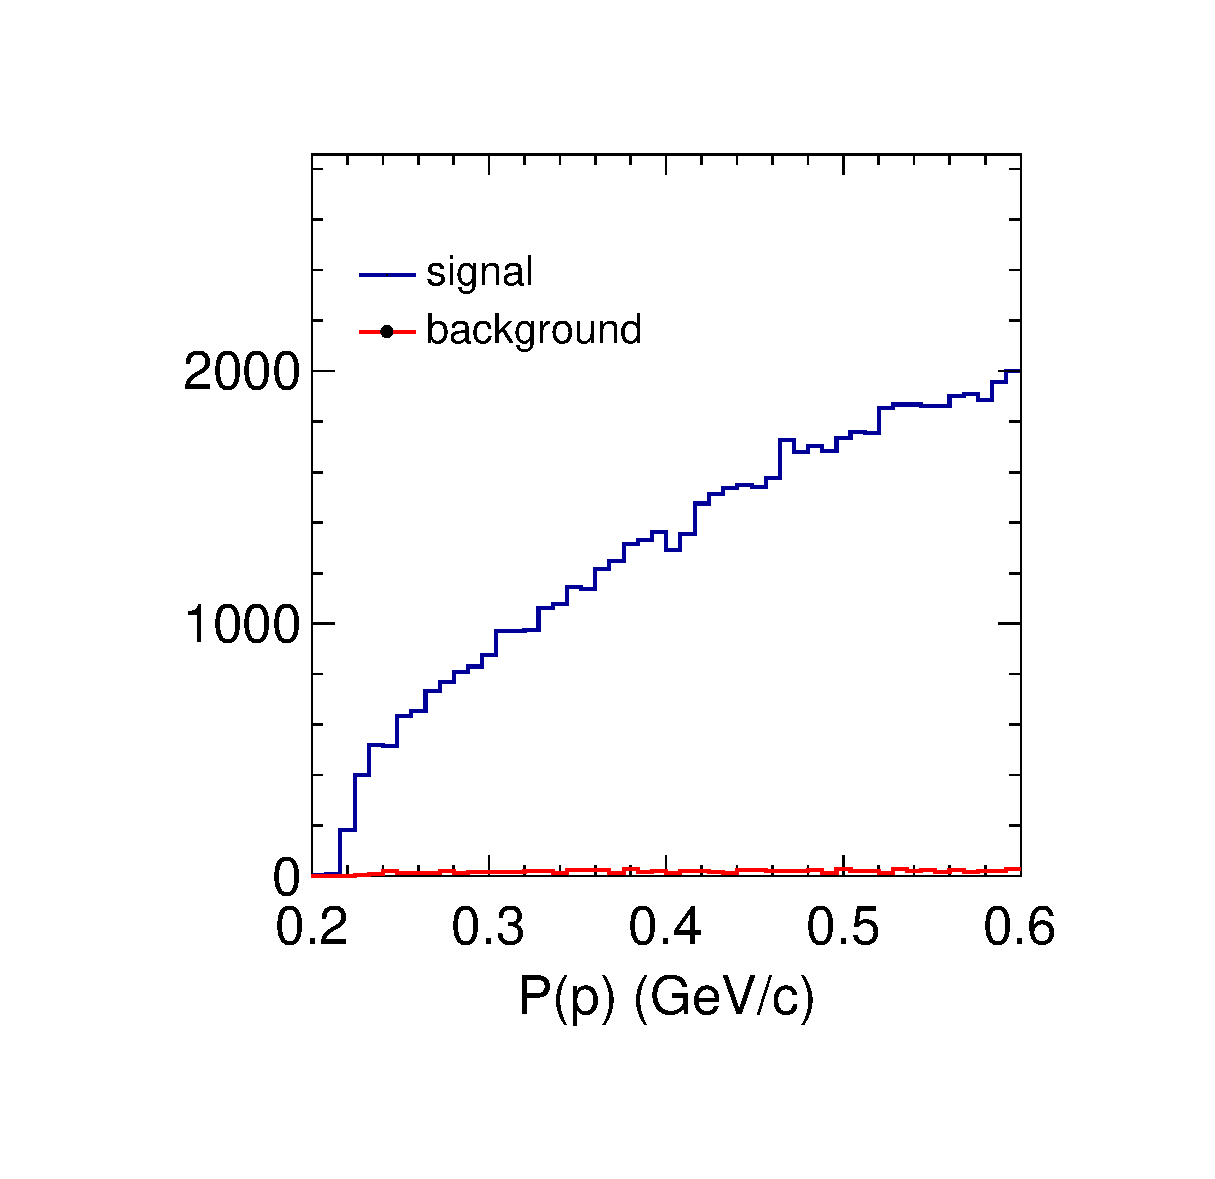
\includegraphics[width = 5 cm]{section/append/fig/momenta_pr_qqmc.eps}
    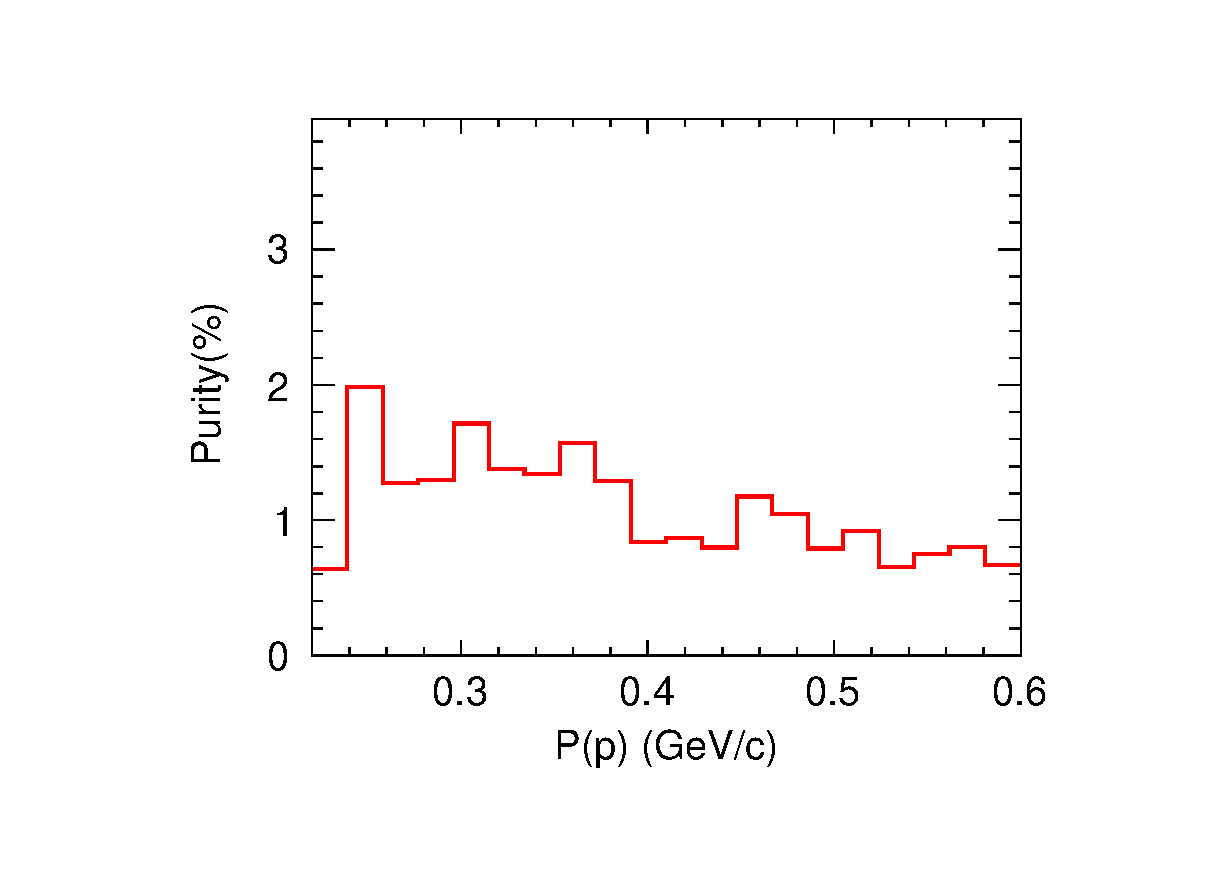
\includegraphics[width = 5 cm]{section/append/fig/Purity_pr_qqmc.eps}
    \caption{质子的动量分布图。红色的实线部分展示了本底的贡献。右图展示了不同动量区间内的信号纯度。
    }\label{Fig:bkg_level_for_proton}
\end{figure}

\subsubsection{PID efficiency}
对正反质子的粒子鉴别的具体条件为:
\begin{itemize}
    \item 利用dEdx和修正后的TOF信息。
    %\item $|\chi| < 9 $
    \item prob~(p) $>$ prob~(K)及 prob~(p) $>$ prob~($\pi$)
\end{itemize}
控制样本中的质子产额及通过粒子鉴别程序的数目均通过拟合丢失质量谱得到,并进一步得到效率。
这里的丢失不变质量$MM^{2}$的定义是:
\begin{equation} 
    MM^{2} = \left( E_{cm} - E_{\bar{p}} - E_{\pi^{+}} -
    E_{\pi^{-}} \right){}^{2} - \left(- p_{\bar{p}} - p_{\pi^{+}} - p_{\pi^{-}} \right)
    {}^{2}
\end{equation}
在对丢失不变质量谱的拟合过程中,模型的构造方式如下。
我们用经过匹配之后的信号蒙特卡洛样本来提取信号形状,并从inclusive 蒙特卡洛样本中
匹配失败的事例提取本底的形状。考虑到粒子鉴别的效率对质子的动量有比较强的依赖,
我们决定将控制样本按动量的大小每隔50MeV划分为若干样本。
而图\ref{Fig:compare_cos_data_MC}显示出控制样本中质子的角分布符合的比较好,
因此不对角度进行分门别类的研究。
\begin{figure}
    \mbox{%
        \begin{overpic}[width = 8 cm]{section/append/fig/Compare_cos_pr_data_Mc.eps}
            \put(75,75) {$(p)$}
        \end{overpic}
        \begin{overpic}[width = 8 cm]{section/append/fig/Compare_cos_antipr_data_Mc.eps}
            \put(75,75) {$(\bar{p})$}
        \end{overpic}
    }
    \caption{数据和蒙特卡洛样本中的质子的$\cos\theta$分布。
    }%
    \label{Fig:compare_cos_data_MC}
\end{figure}
\subsubsection{质子粒子鉴别效率}
如图\ref{fig:pass_PID},\ref{fig:not_pass_PID}所示,我们通过拟合丢失质量
谱来确定控制样本中质子的数目及相应的通过粒子鉴别程序的个数。
对各个区间的的控制样本进行如此操作后便d分别得到数据和蒙特卡洛样本中的鉴别
效率。图\ref{fig:diff_PID_efficeincy}展示的每个区间内的差别。
受统计量限制,并未发现数据和蒙特卡洛之间的显著差别。
\begin{figure}[htbp]
    \mbox{%
        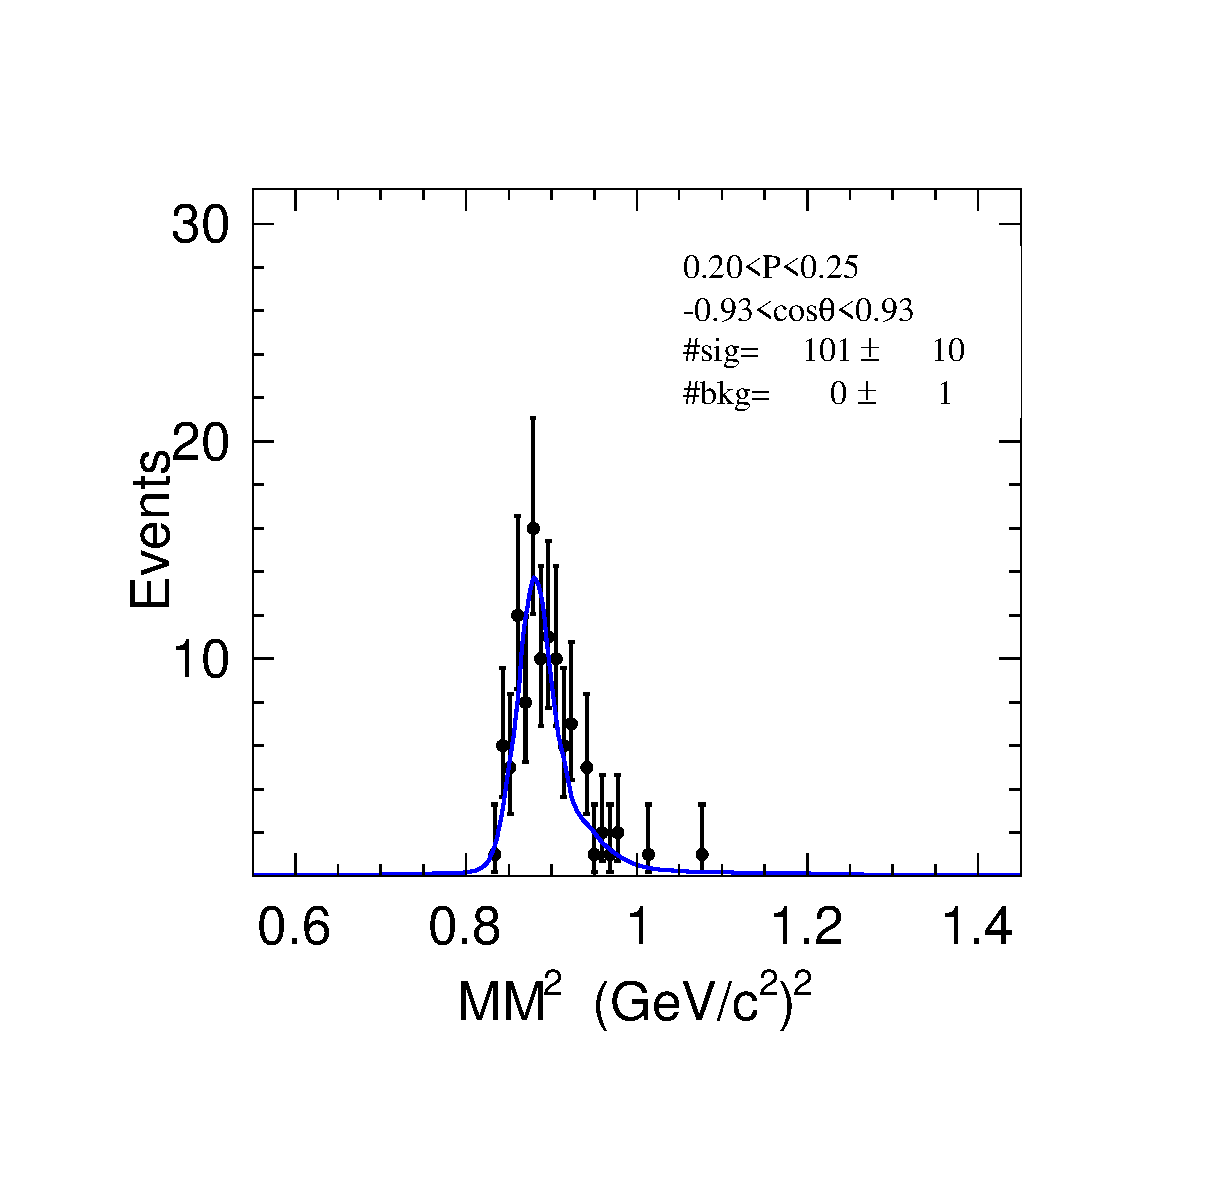
\includegraphics[width = 5 cm]{section/append/fig/Plot_MMSq_0_0_data.eps}  
        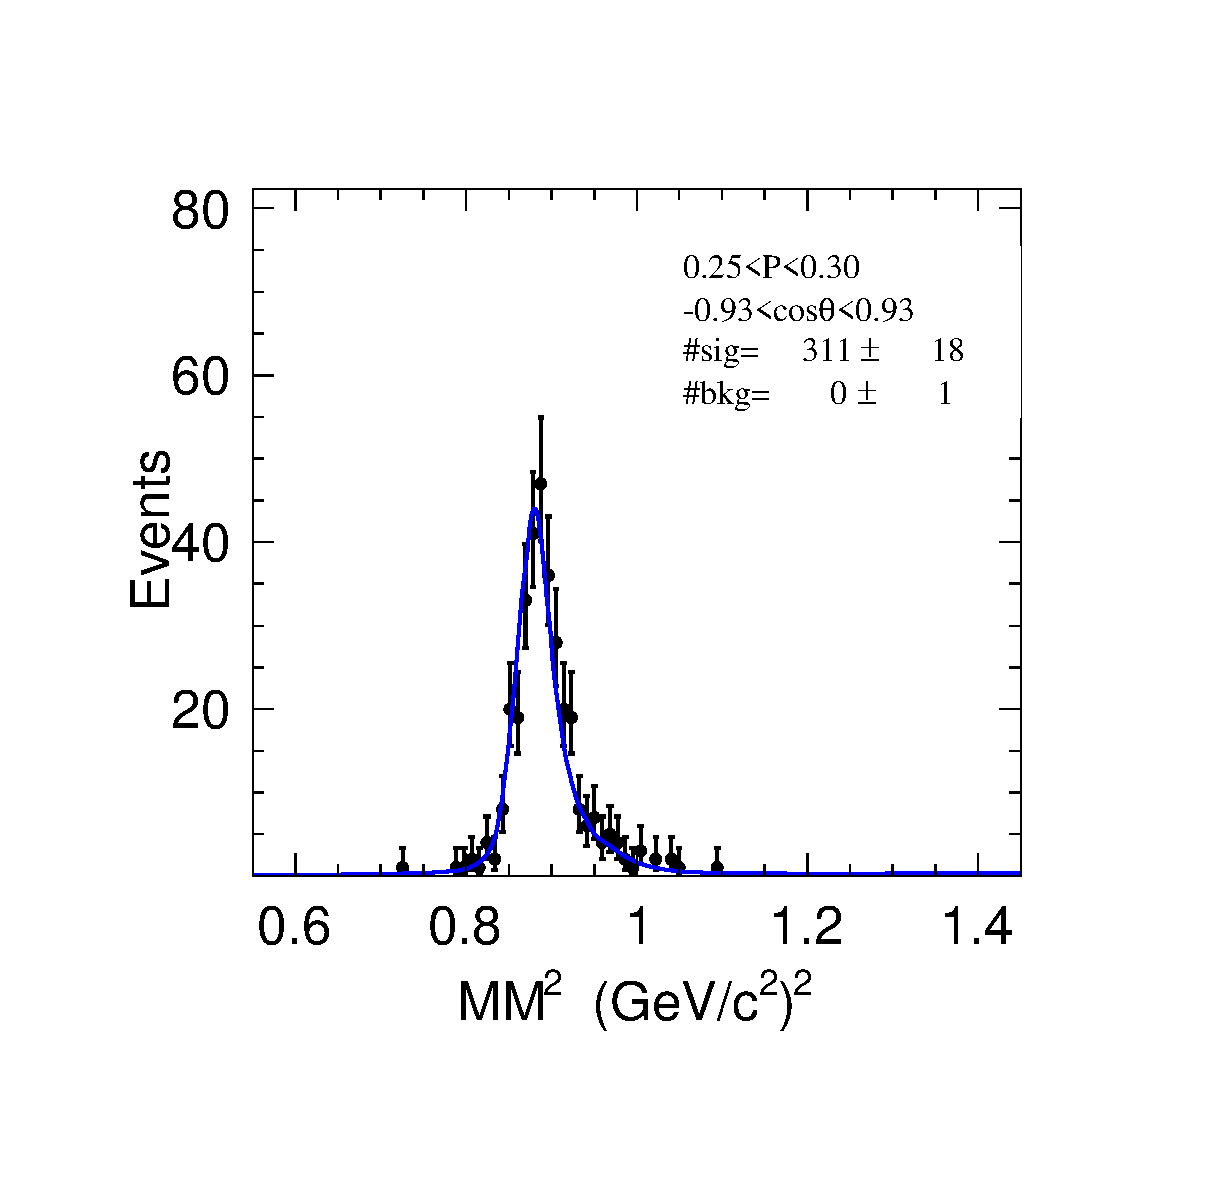
\includegraphics[width = 5 cm]{section/append/fig/Plot_MMSq_1_0_data.eps}
        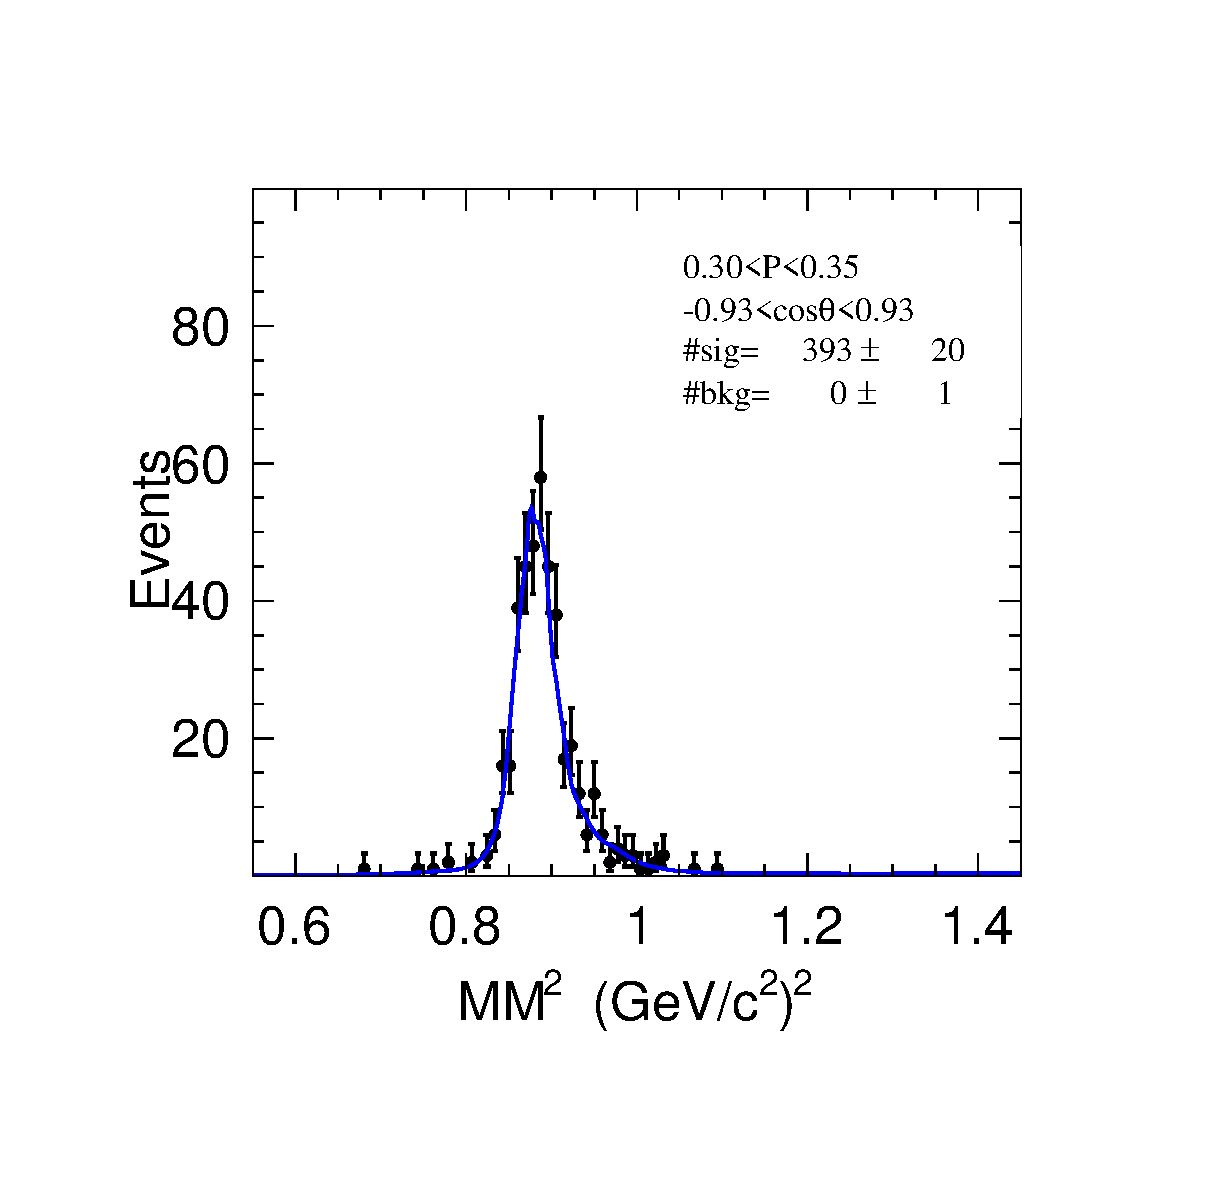
\includegraphics[width = 5 cm]{section/append/fig/Plot_MMSq_2_0_data.eps}       
    }
    \mbox{%
        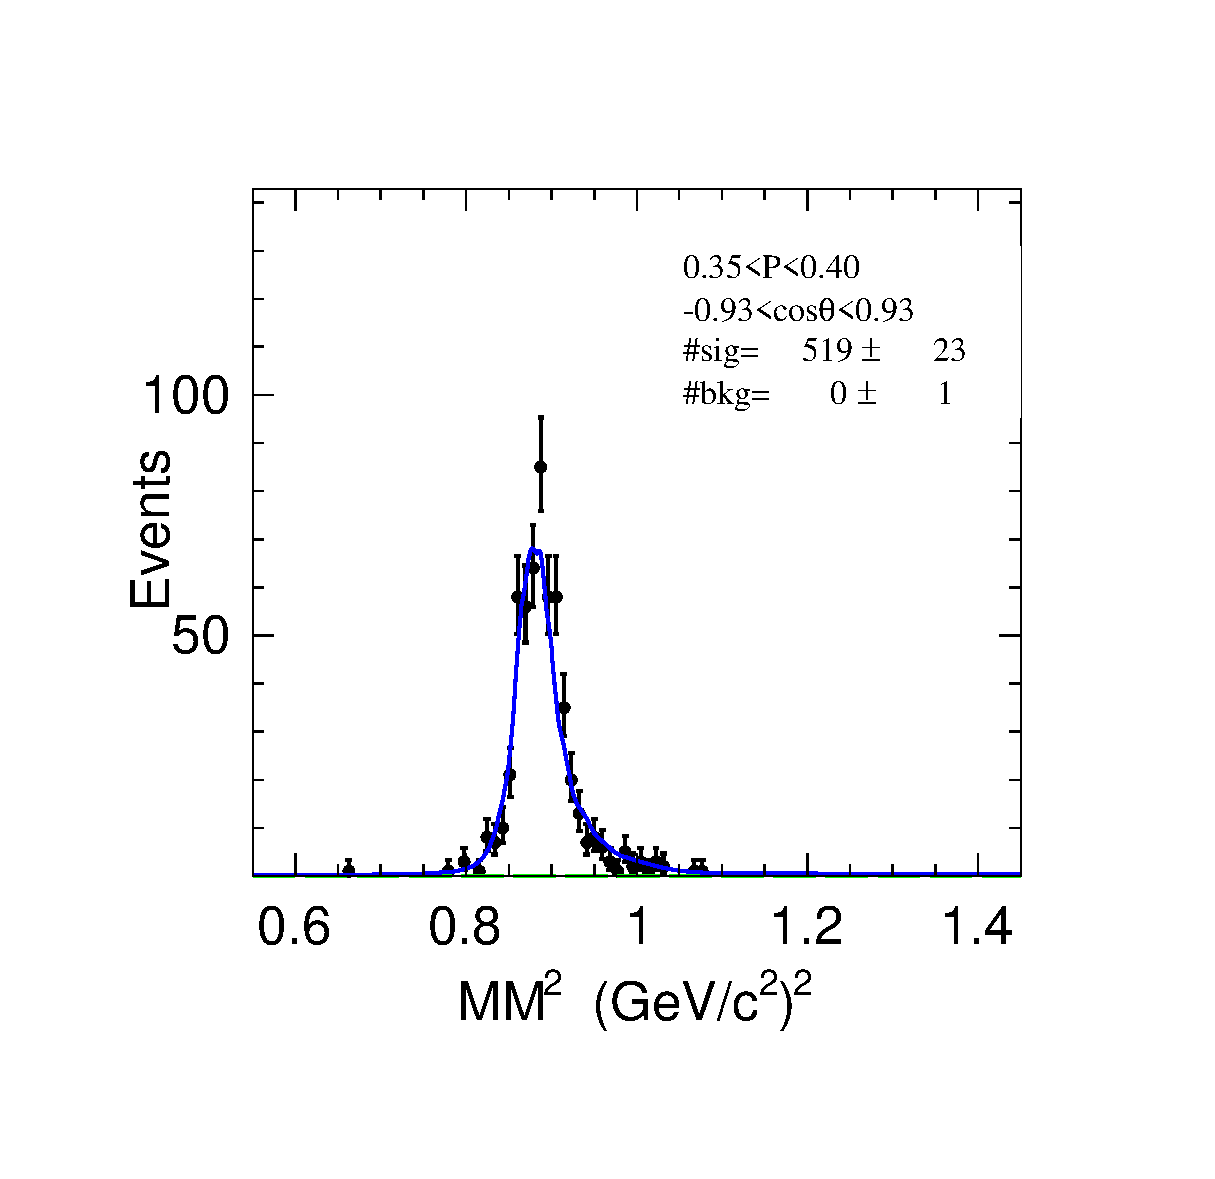
\includegraphics[width = 5 cm]{section/append/fig/Plot_MMSq_3_0_data.eps}  
        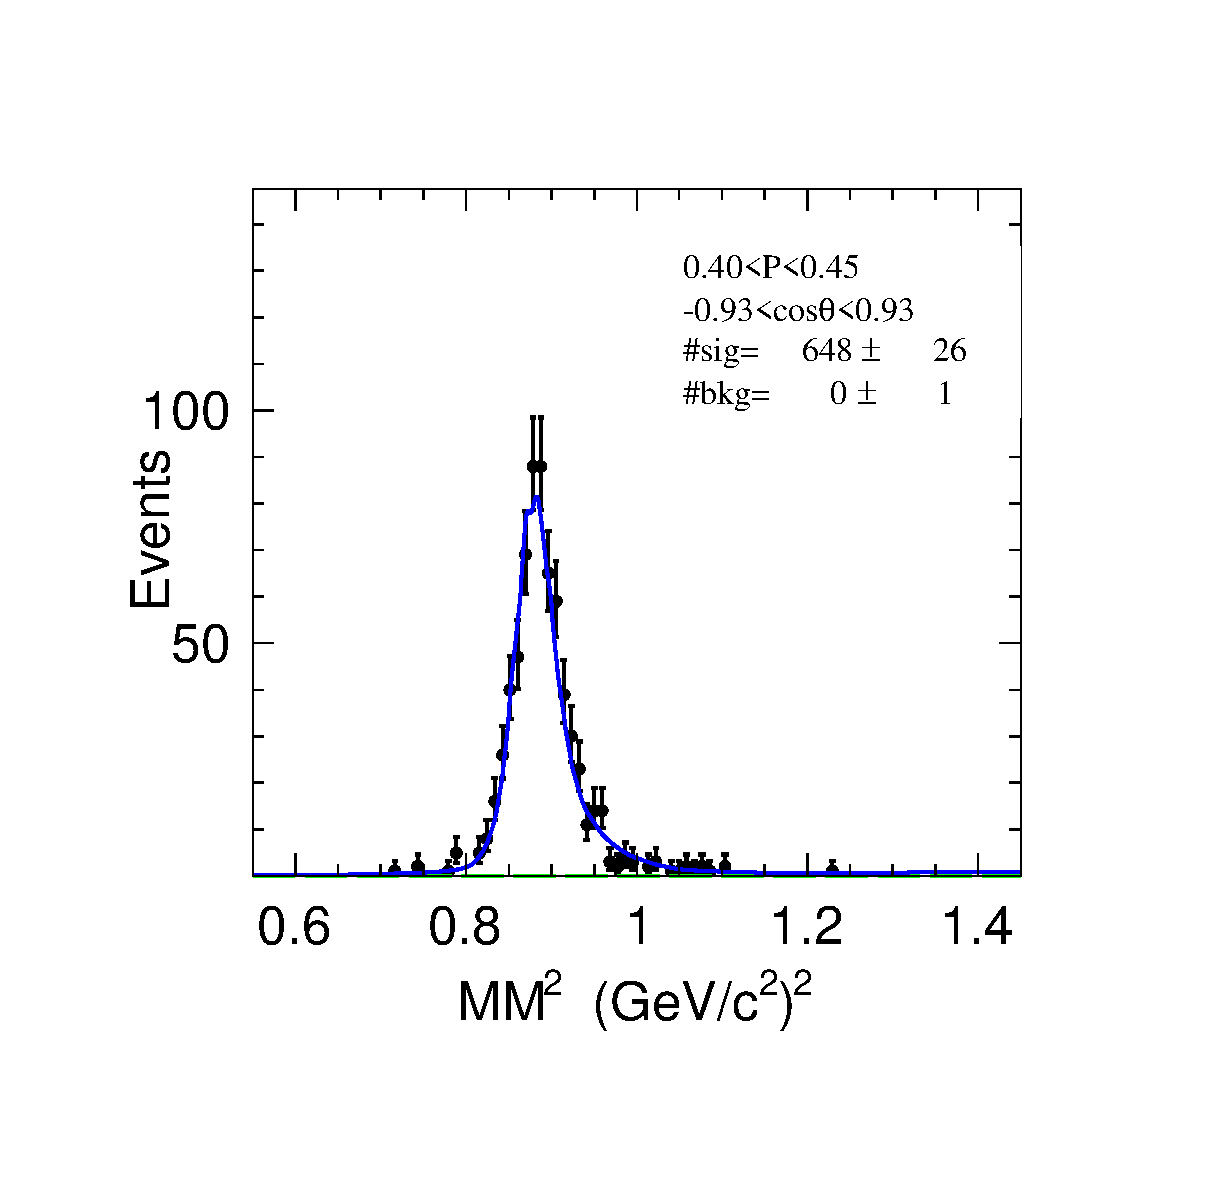
\includegraphics[width = 5 cm]{section/append/fig/Plot_MMSq_4_0_data.eps}
        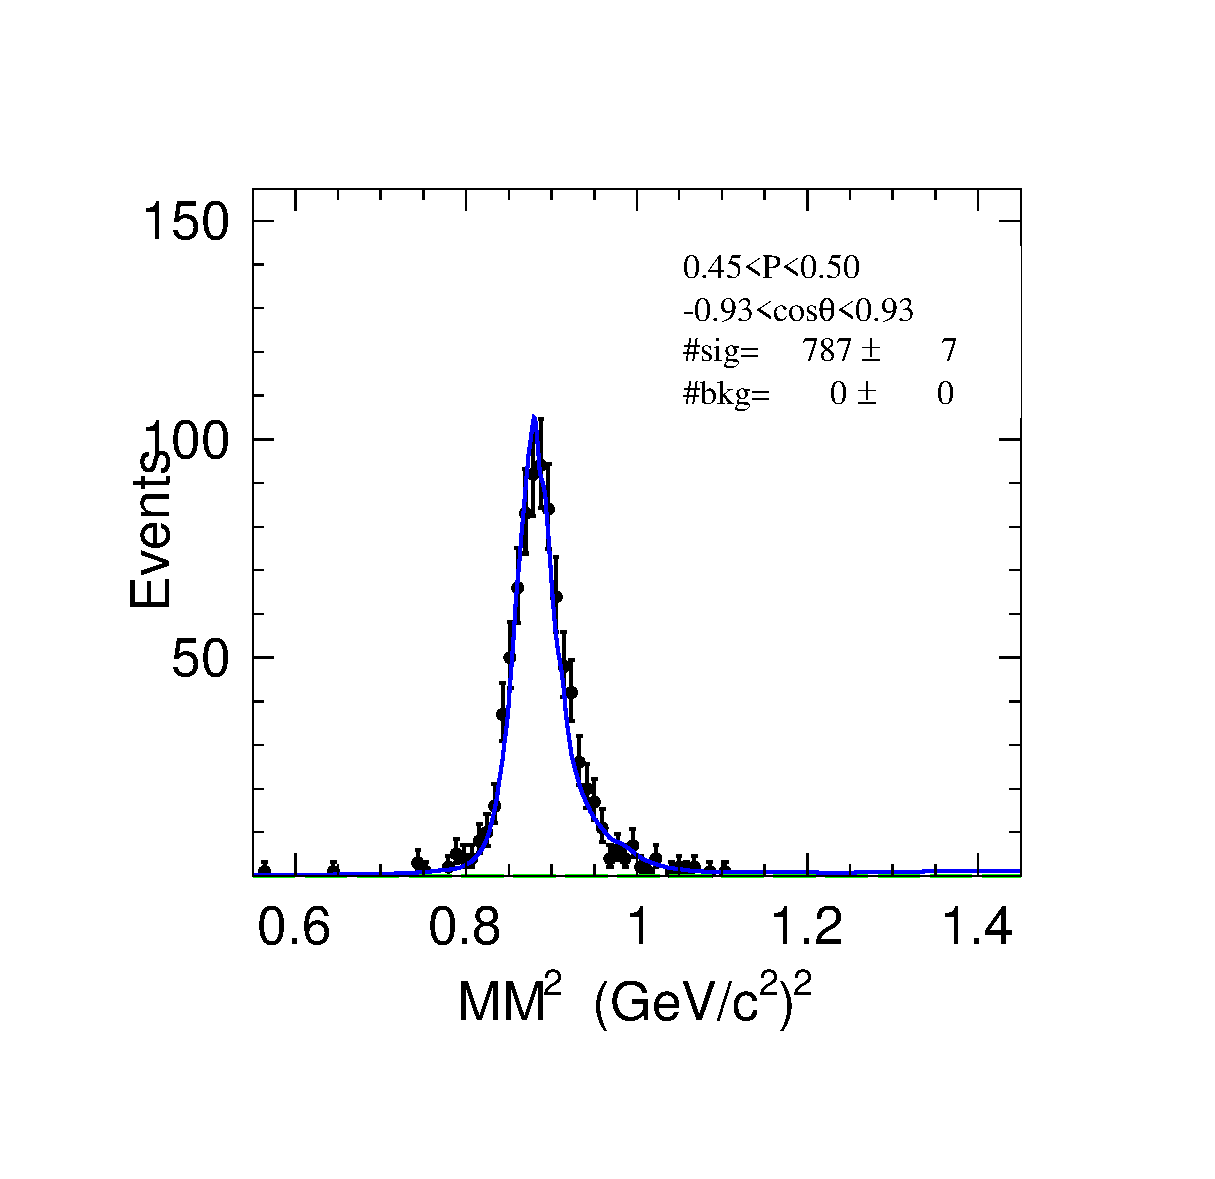
\includegraphics[width = 5 cm]{section/append/fig/Plot_MMSq_5_0_data.eps}       
    }
    \caption{每个区间内的通过粒子鉴别的质子的个数。}%
    \label{fig:pass_PID}
\end{figure}

\begin{figure}[htbp]
    \mbox{%
        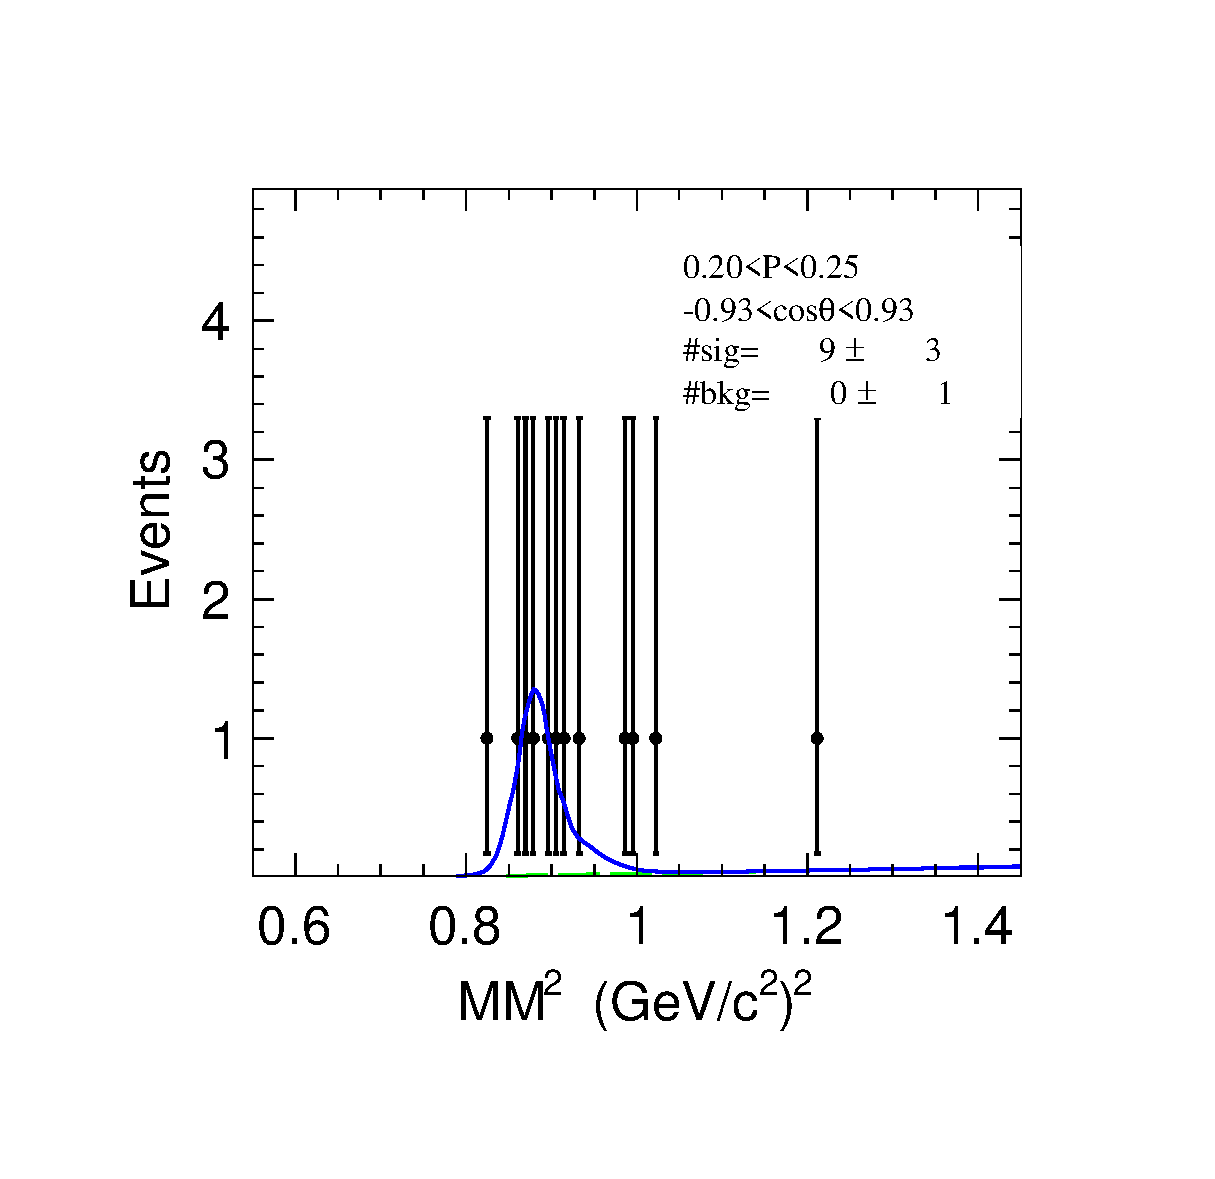
\includegraphics[width = 5 cm]{section/append/fig/Plot_MMSq_unpid_0_0_data.eps}  
        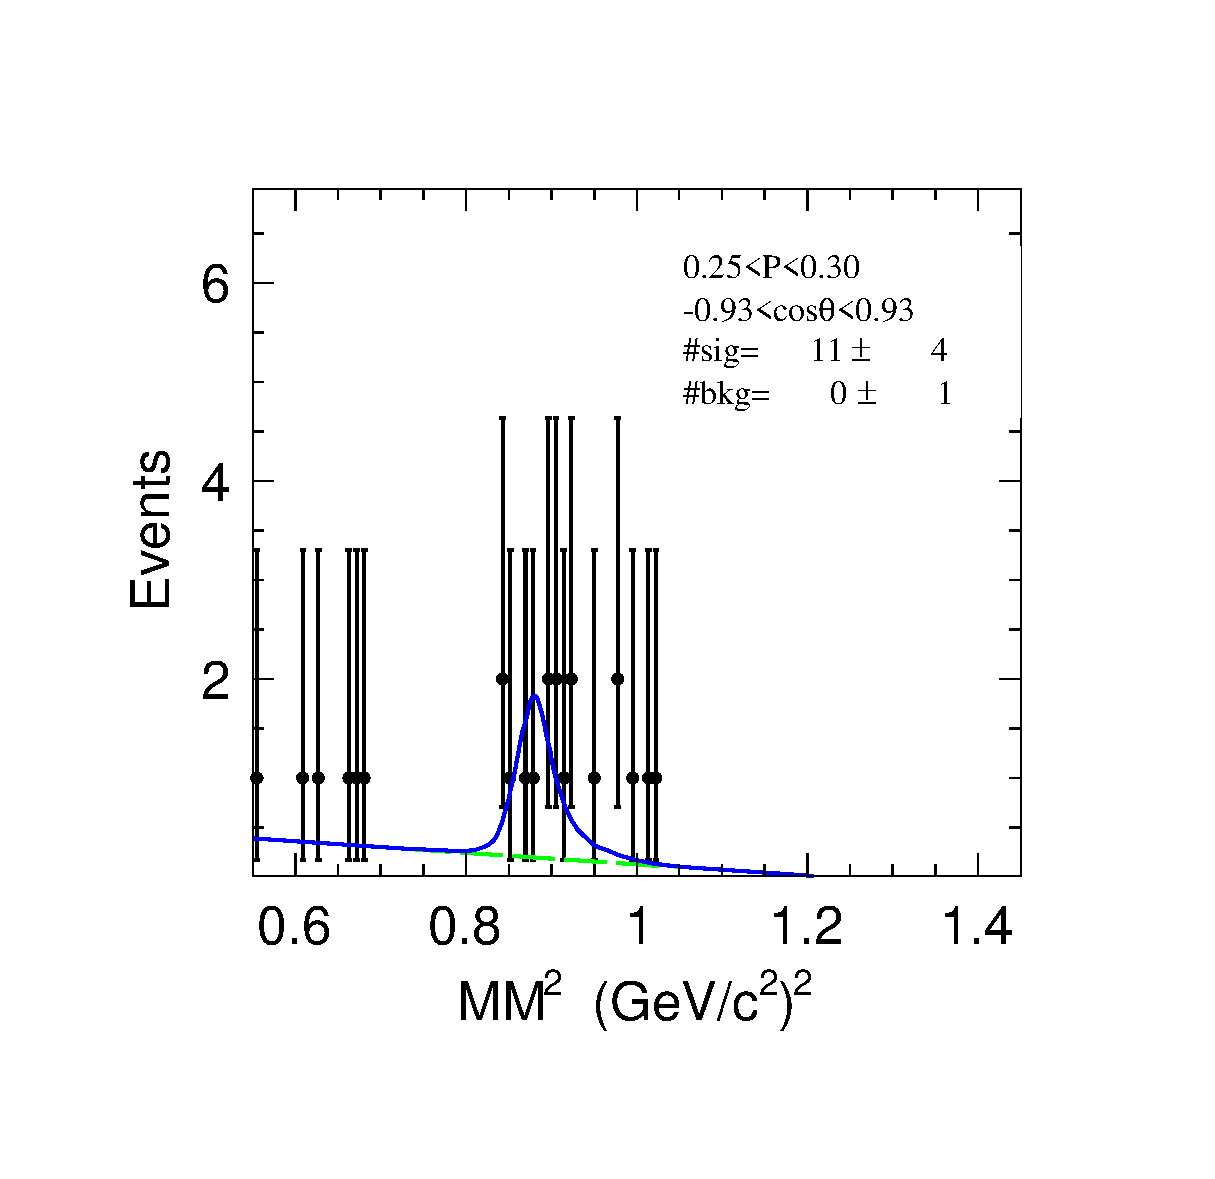
\includegraphics[width = 5 cm]{section/append/fig/Plot_MMSq_unpid_1_0_data.eps}
        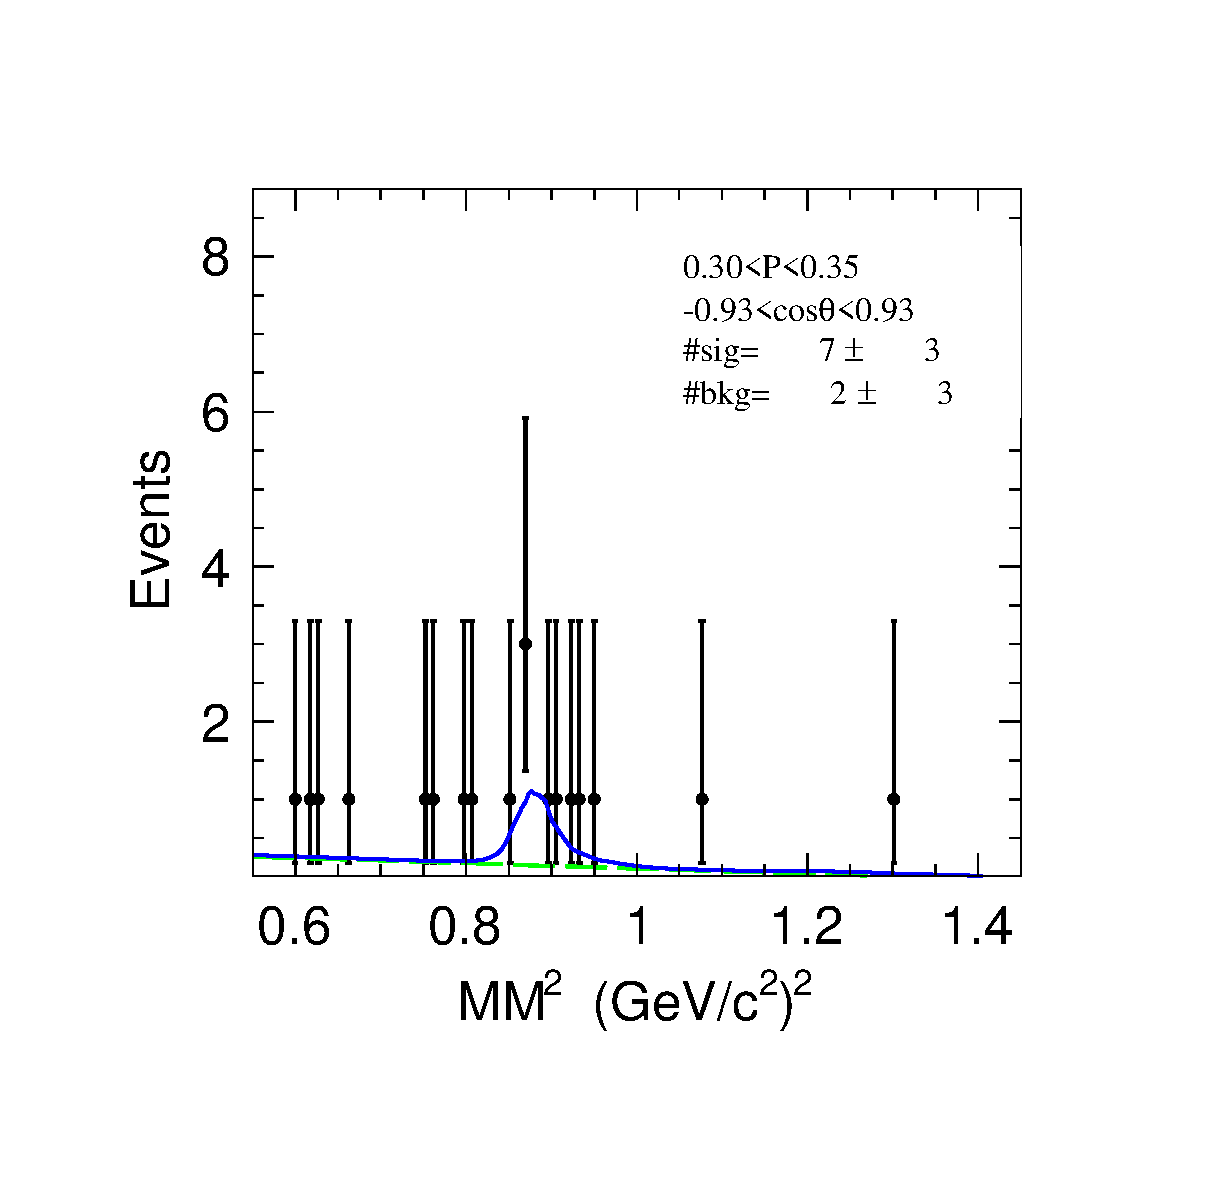
\includegraphics[width = 5 cm]{section/append/fig/Plot_MMSq_unpid_2_0_data.eps}       
    }
    \mbox{%
        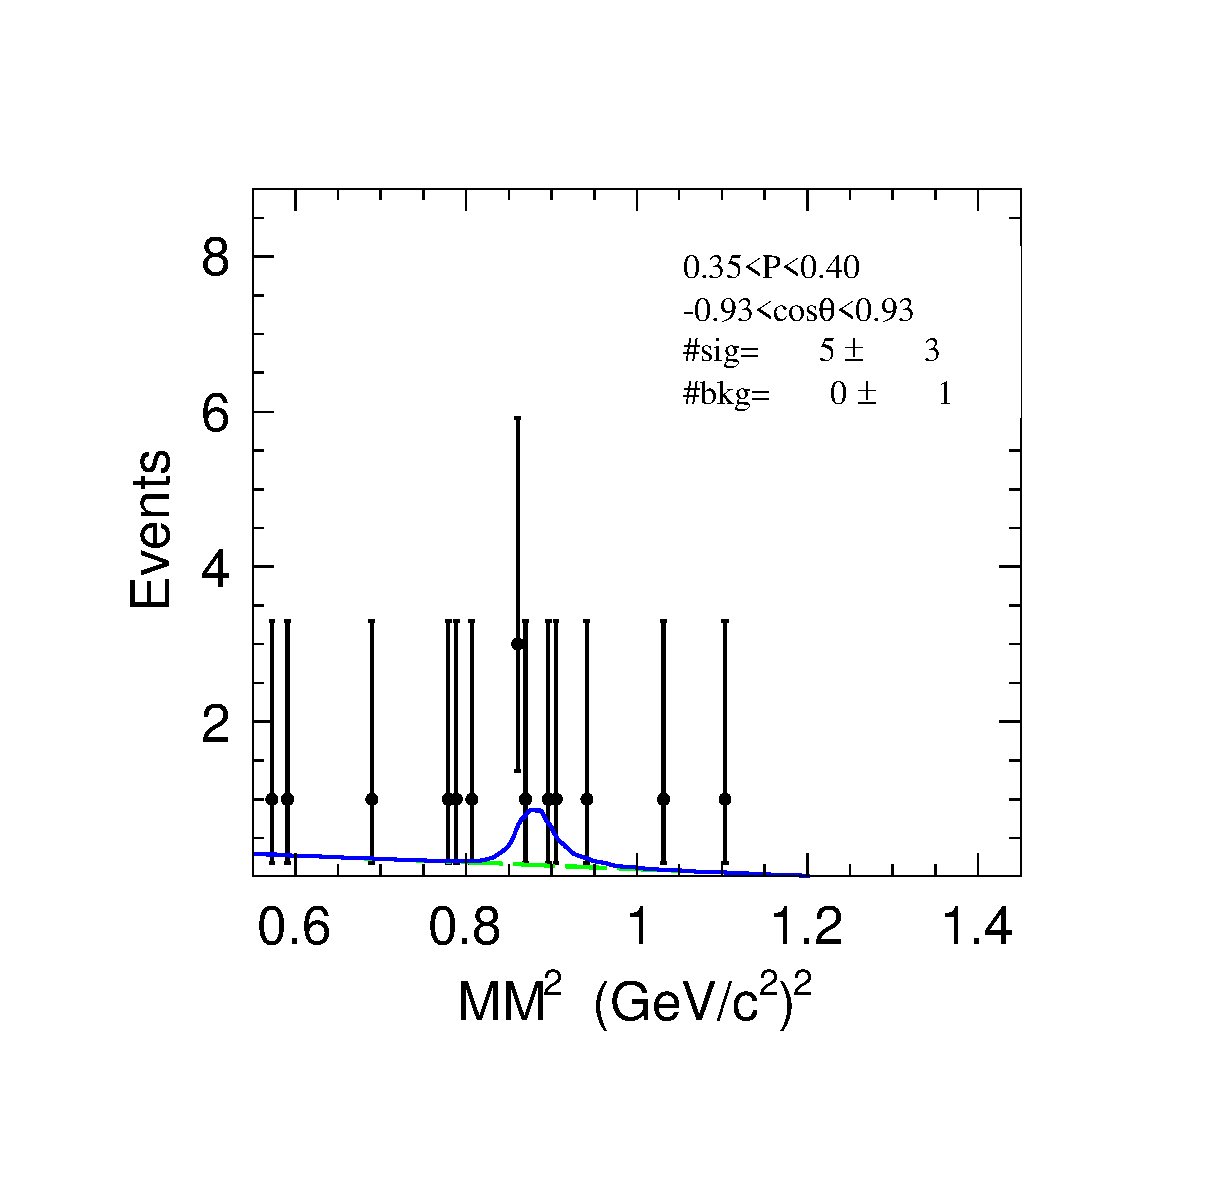
\includegraphics[width = 5 cm]{section/append/fig/Plot_MMSq_unpid_3_0_data.eps}  
        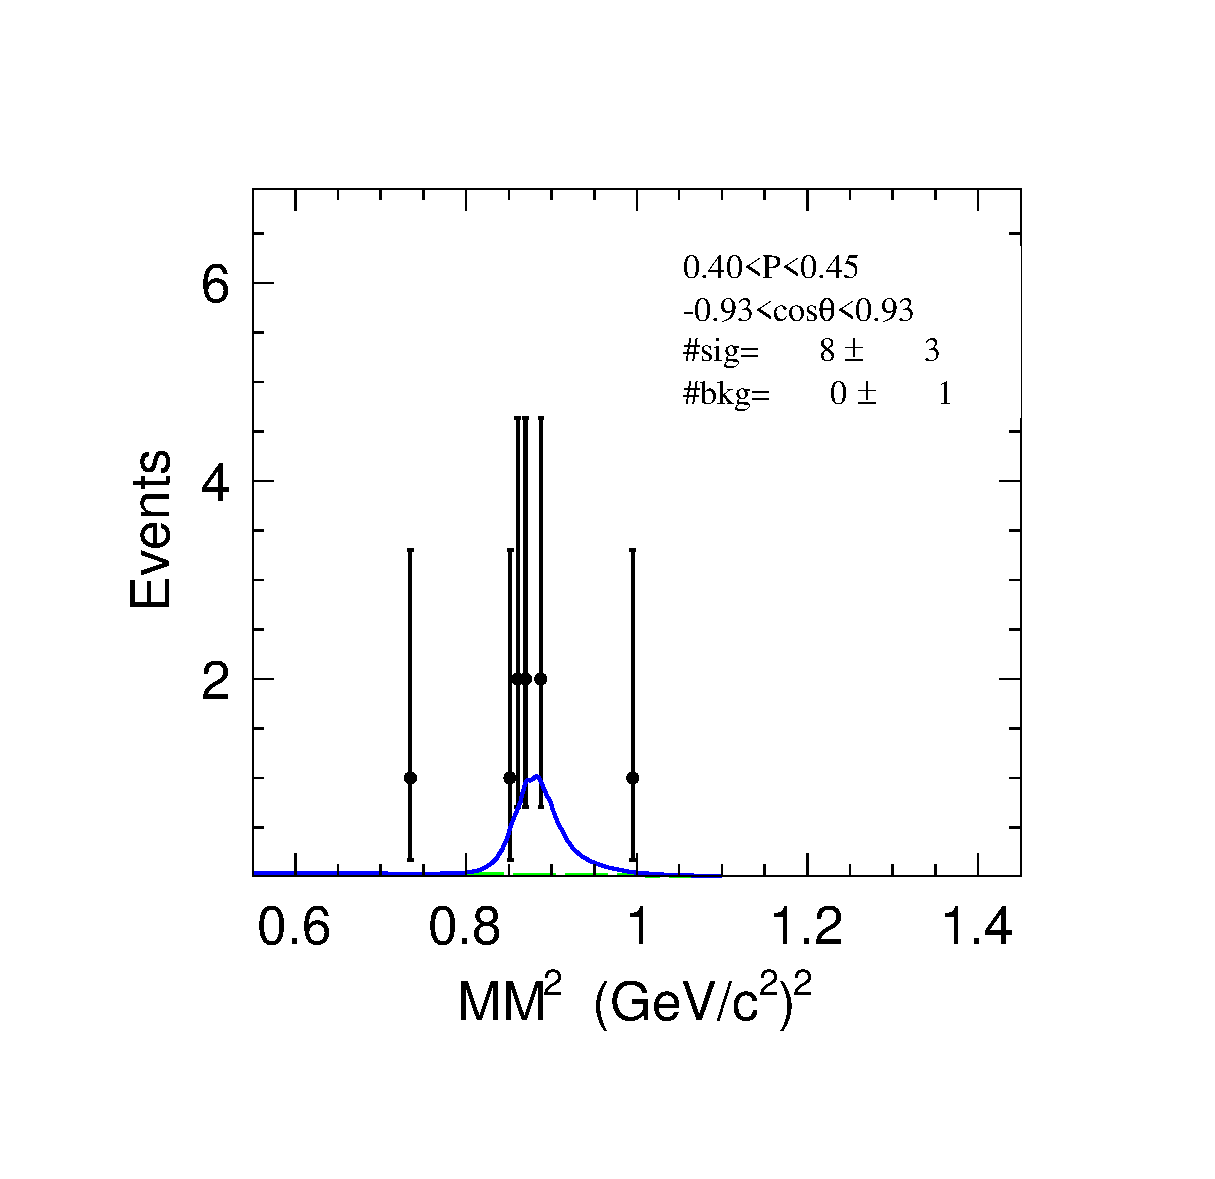
\includegraphics[width = 5 cm]{section/append/fig/Plot_MMSq_unpid_4_0_data.eps}
        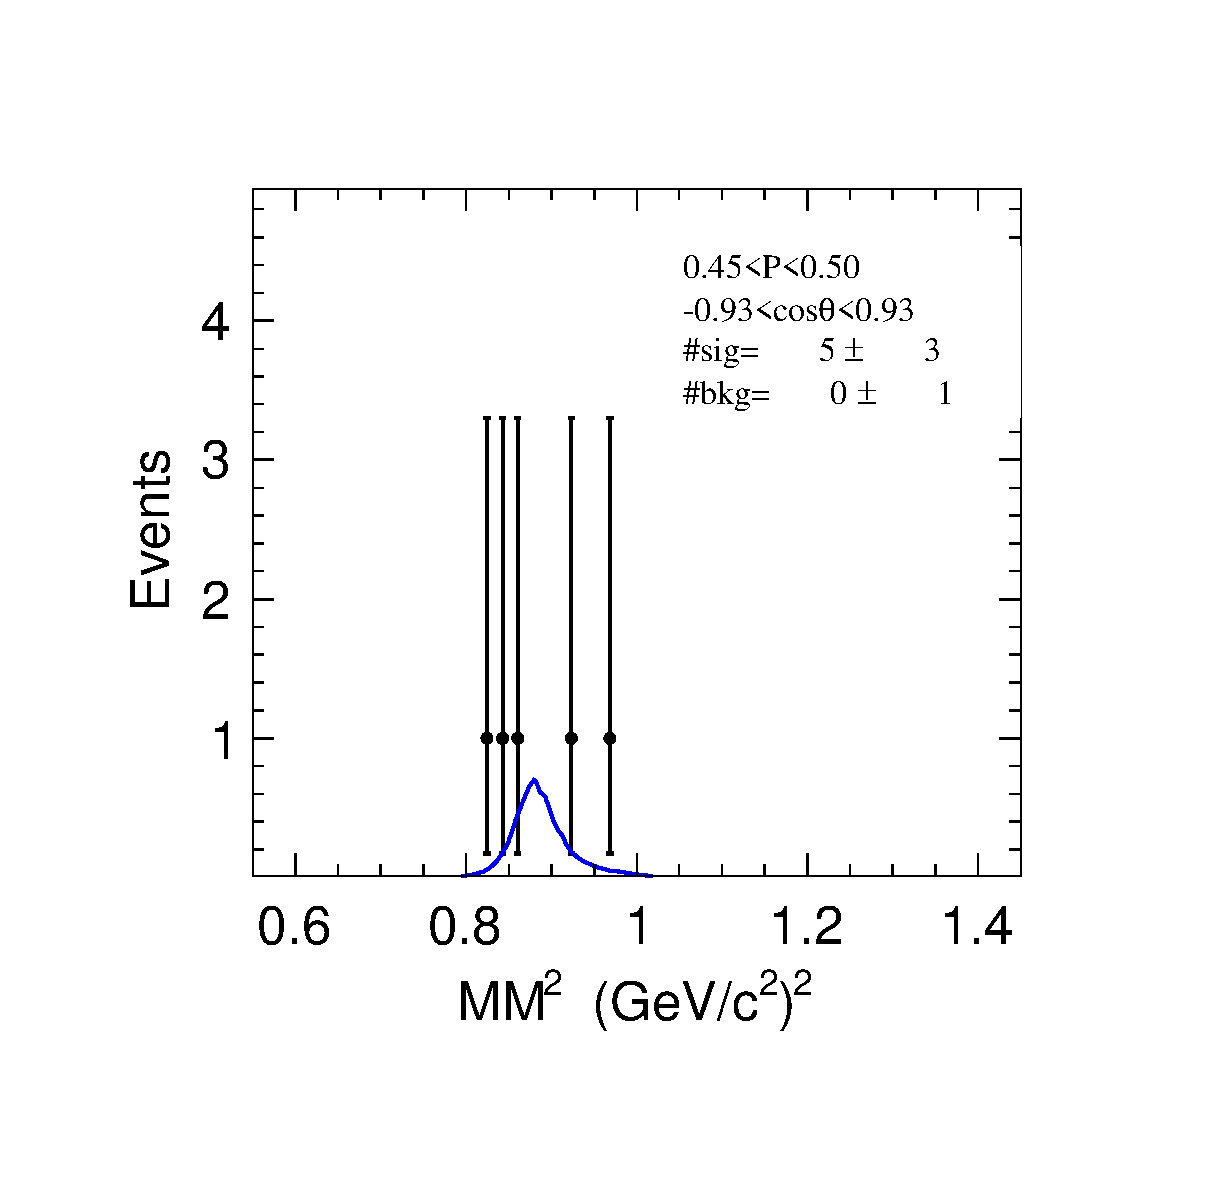
\includegraphics[width = 5 cm]{section/append/fig/Plot_MMSq_unpid_5_0_data.eps}       
    }
    \caption{每个区间内的没有通过粒子鉴别的质子总数。}%
    \label{fig:not_pass_PID}
\end{figure}

\begin{figure}[htbp]
    \mbox{%
        \begin{overpic}[width = 8 cm]{section/append/fig/Compare_eff_data_MC_pr.eps}     
            \put(75,75) {$(p)$}    
        \end{overpic}
        \begin{overpic}[width = 8 cm]{section/append/fig/Compare_eff_data_MC_antiPr.eps}     
            \put(75,75) {$(\bar{p})$}    
        \end{overpic}
    }
    \caption{数据和蒙特卡洛样本间的粒子鉴别效率的差异。
    蓝色和红色的数据点分别代表数据中
    和蒙特卡洛中的效率。}%
    \label{fig:diff_PID_efficeincy}
\end{figure}
